\section{Sơ đồ nguyên lý}
\subsection{Vi điều khiển PIC16F887}
\begin{figure}[H]
    \centering
    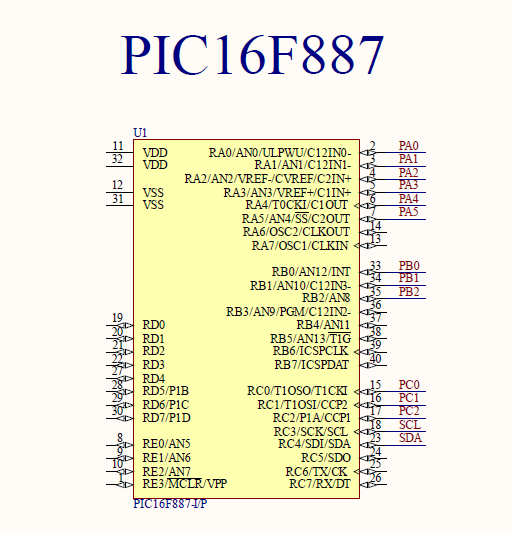
\includegraphics[width=0.7\textwidth]{pictures/pic_sch.png}
\end{figure}
Là trung tâm xử lý điều khiển toàn bộ hệ thống. Các chân I/O của vi điều khiển được cấu hình để:
\begin{itemize}
    \item Giao tiếp với LED qua IC dịch 74HC595.
    \item Đọc trạng thái nút nhấn để chuyển chế độ.
    \item Giao tiếp LCD qua giao tiếp I2C (sử dụng module PCF8574).
\end{itemize}
Các chân của vi điều khiển được sử dụng trong mạch như sau:
\begin{itemize}
    \item \texttt{RA0 -- RA5}: Điều khiển các cụm đèn LED giao thông (đỏ, vàng, xanh) cho từng hướng.
    \item \texttt{RB0 -- RB2}: Nhận tín hiệu từ 3 nút nhấn dùng để chuyển chế độ hoạt động và chuyển pha đèn trong chế độ thủ công.
    \item \texttt{RC3 (SCL)} và \texttt{RC4 (SDA)}: Giao tiếp I2C với module PCF8574T để điều khiển LCD 1602.
    \item \texttt{RC0 -- RC2}: Giao tiếp với IC 74HC595 để đồng bộ hóa dữ liệu xuất ra LED 7 đoạn.
\end{itemize}

\subsection{IC dịch 74HC595 và mạch hiển thị 7 đoạn}
\begin{figure}[H]
    \centering
    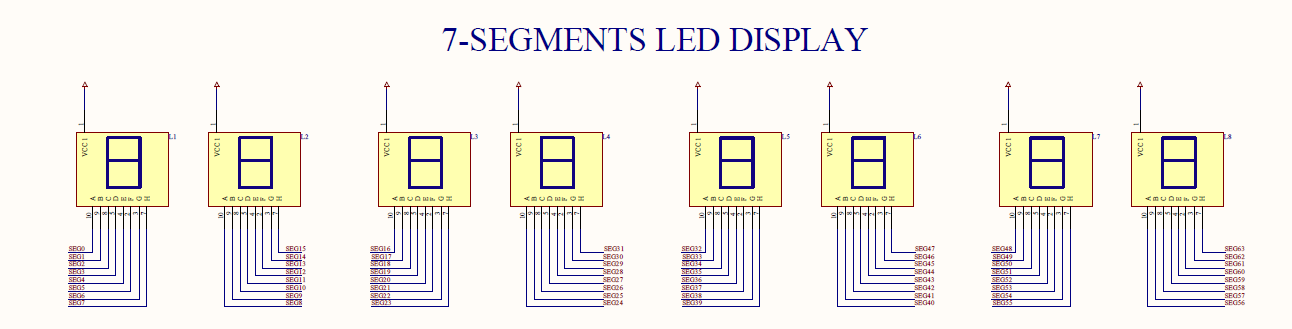
\includegraphics[width=1\textwidth]{pictures/7seg1.png}
\end{figure}
\begin{figure}[H]
    \centering
    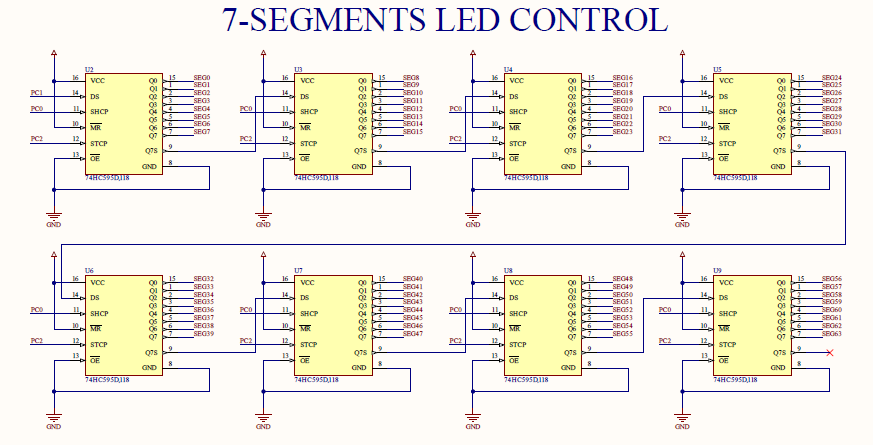
\includegraphics[width=1\textwidth]{pictures/7seg2.png}
\end{figure}
Để tiết kiệm chân I/O của vi điều khiển, hệ thống sử dụng 8 IC 74HC595 để điều khiển nhiều LED 7 đoạn hiển thị đếm ngược thời gian cho các pha đèn. Mỗi IC điều khiển một cụm 8 LED. Cách hoạt động như sau:
\begin{itemize}
    \item Dữ liệu nhị phân từ PIC được dịch nối tiếp qua các IC 74HC595.
    \item Các chân \texttt{SHCP}, \texttt{STCP} và \texttt{DS} được điều khiển nhịp nhàng để đẩy dữ liệu ra song song.
    \item Tín hiệu hiển thị số được mã hóa theo bảng BCD và cập nhật liên tục theo từng pha đèn.
\end{itemize}

\subsection{LCD 1602 giao tiếp I2C}
\begin{figure}[H]
    \centering
    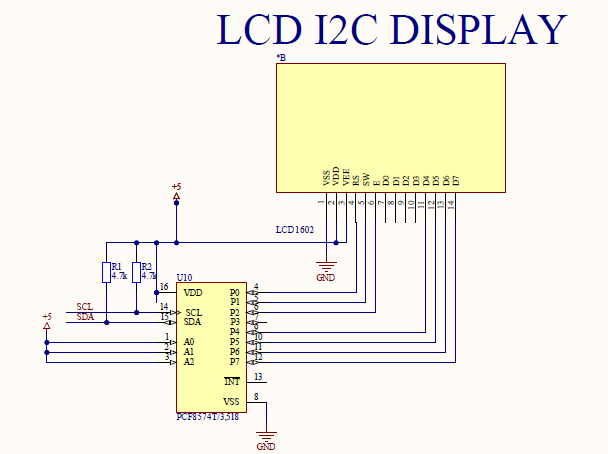
\includegraphics[width=0.7\textwidth]{pictures/lcd_sch.png}
\end{figure}

Màn hình LCD dùng để hiển thị chế độ hiện tại của hệ thống: AUTO MODE, MANUAL MODE, hay NIGHT MODE. Module I2C giao tiếp LCD cho phép điều khiển LCD chỉ với 2 dây:
\begin{itemize}
    \item \texttt{SDA (RC4)}: Truyền dữ liệu.
    \item \texttt{SCL (RC3)}: Truyền xung clock.
\end{itemize}
Sử dụng mô dun giao tiếp LCD I2C giúp giảm số lượng chân cần sử dụng, từ 6--8 chân xuống còn 2, rất hữu ích cho các hệ thống có số lượng chân giới hạn.
